\chapter{Literatuur}

\begin{itemize}
		\item Bron \cite{Review-of-Action-Recognition-and-Detection-Methods}
	\begin{itemize}
		\item Actieherkenning = het herkennen van een actie binnen een goed gedefinieerde omgeving 
		\item Actiedetectie = het herkennen en lokaliseren van acties(begin, duratie en einde) in de ruimte en de tijd
		\item training set = wordt gebruikt om classifier te trainen
		\item validation set = optioneel, bevat andere data dan de training set om de classifier te optimaliseren
		\item testing set = testen van de classifier (performance)
		\item Drie manieren om dataset op te splitsen in deze drie sets:
		\begin{itemize}
			\item voorgedefinieerde split: De dataset wordt opgesplitst  in twee of drie delen zoals de auteurs van die dataset dat vermelden
			\item n-voudige cross-validatie: Verdeeld de dataset in n gelijkvoudige stukken. Hierbij worden er (n-1)/n  percentage van de videos gebruikt om te trainen, en dan de overige 1/n om te testen. Dit proces wordt n keer herhaald, zodat elke video éénmaal gebruikt werd voor te testen
			\item leave-one-out cross-validatie:
		\end{itemize}
		
		
		\item  om actieklasse te bepalen = features extraheren en in classifier steken => classifier bepaalt actieklasse
		\item Temporally untrimmed video = delen van de video bevatten GEEN ENKELE actie. Variaties van dezelfde actie kan op hetzelfde moment voorkomen
		
		\item THUMOS challenge:
		\item 2015 => slechts één team heeft detection challenge geprobeerd
		
		\item 	Classificatietaak: de lijst van acties geven die in een lange, niet getrimde video voorkomen
		\item 	Detectietaak: ook de lijst van acties geven PLUS de plaats in tijd waar ze voorkomen
	\end{itemize}

	\item Bron \cite{real-time-human-pose-recognition-in-parts-from-a-single-depth-image}
	gaat eerder over hoe het skelet bepaalt wordt
	\begin{itemize}
		\item voorstel van een methode om op een accurate manier de 3D posities van de joints te bepalen, vanuit slechts één dieptebeeld, zonder temporale informatie
		\item Het bepalen van lichaamsdelen is invariant van pose, lichaamsbouw, kleren, etc...
		\item Kan runnen aan 200 fps
		\item Wordt effectief gebruikt in de Kinect software (onderzoeksteam is van Microsoft)
		\item Een dieptebeeld wordt gesegmenteerd in verschillende lichaamsdelen, aangegeven door een kleur, op basis van een kansfunctie; Elke pixel van het lichaam wordt apart behandeld en gekleurd. Een verzameling van dezelfde kleuren wordt een joint
		\item Aangezien tijdsaspect weg is, is er enkel interesse in de statische poses van een frame. Verschillen van pose in twee opeenvolgende frames is miniscuul zodat die genegeerd worden
	\end{itemize}

	\item Bron \cite{xia2012view}
	\begin{itemize}
		\item[$\vee$] Bevat bruikbare datasets van skelet-, diepte- en kleurenbeelden
		\item Ook hier praten ze over de vaak voorkomende uitdagingen: Intra-en interklasse variaties, de omgeving en de grootte van de verzameling van acties die er eigenlijk bestaan.
		\item Hier tonen ze ook weer het nut van de kinect sensor aan, en gebruiken de kinect
		\item Ze geven een nieuw algoritme om menselijke actieherkenning uit te voeren vanuit een dieptebeeld, een view-invariante representatie van poses en het systeem werkt \underline{real-time}. 
		
		{\color{red}! Het real-time component bevat drie zaken:
			\begin{itemize}
				\item Het verkrijgen van de 3D locaties van de joints $\rightarrow$ via bron \cite{real-time-human-pose-recognition-in-parts-from-a-single-depth-image}
				\item Het berekenen van HOJ3D (histogram)
				\item Classificatie
			\end{itemize} }
		\item Histogram gebaseerde representatie van 3D poses (HOJ3D genoemd) = partitie van 3D ruimte in $n$ "bins", gebruik maken van een bolcoördinatensysteem. Selectie van 12 joints die een compacte representatie van het skelet weergeven. (hand en pols, voet en enkel worden gecombineerd).
		\item Het centrum van deze 3D ruimte is de de heup joint. Er is ook een vector $\alpha$, parallel met de grond, door de heup (van links naar rechts), en een vector $\theta$ loodrecht op de grond en door het centrum
			\begin{figure}[ht]
				\centering
			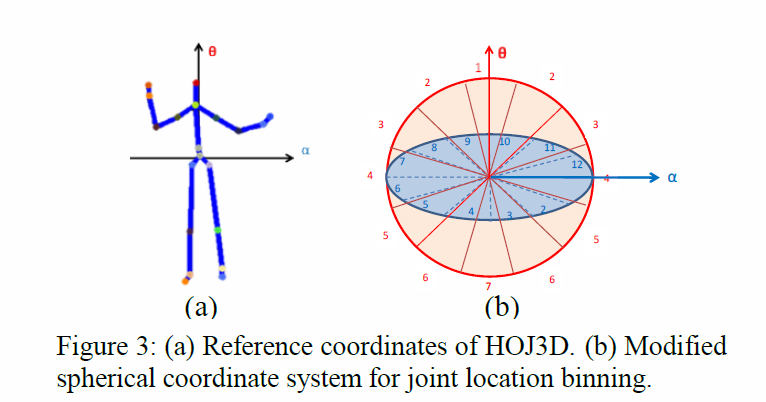
\includegraphics[width=\textwidth]{HOJ3D}
			\end{figure}
			Deze 3D ruimte (figuur 3b) wordt opgesplitst in $n$ partities.
			
			Voor $\theta$: [0, 15], [15, 45], [45, 75], [75, 105] [105, 135], [165, 180]. (7 bins)
			
			Voor $\alpha$: 30 graden voor elke bin, dus 12 bins.
			
			in totaal $7 * 12 = 84$ bins
		
			
			Via deze bolcoördinaten kan elke 3D joint gelokaliseerd worden in een unieke bin 
			\item De 3 joints die gebruikt worden om het bolcoördinatenstelsel te oriënteren staan uiteraard vast. De overige 9 joints worden onderverdeeld in één van de 84 bins. 
			
			\item Om de representatie robust te maken, wordt één enkele joint over verschillende, naburige bins verdeeld (8 buren), op basis van gewichtsfunctie:

			
			\begin{figure}[ht]
				\centering
				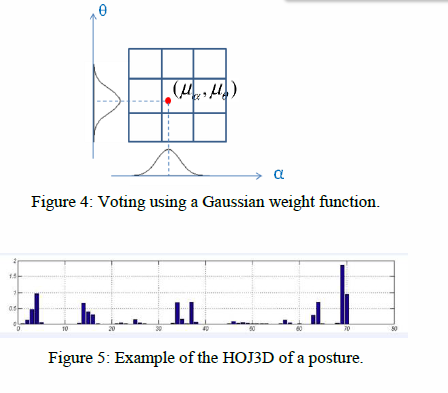
\includegraphics[width=0.5\textwidth]{HO3D_HISTOGRAM}
			\end{figure}
			
			\item Linear discriminant analysis (LDA) wordt toegepast om dominante features eruit deze histogram te halen.
			
			\item Ze stellen voor om kleurenbeelden te combineren met dieptebeelden om algoritmen te ontdekken met beter herkenning
			
			\item Ze beweren sneller te zijn dan bron \cite{action-recognition-based-bag-3d-points}
		\end{itemize}
	\item Bron \cite{action-recognition-based-bag-3d-points} (pre-kinect era)
	\begin{itemize}
		\item Actieherkenning met behulp van reeksen van dieptebeelden
		\item Gaan ervan uit dat efficiënte tracking van skeletbeelden nog niet mogelijk is. (is gepubliceerd zelfde jaar dat Kinect beschikbaar was, 2010)
		\item Hun oplossing is dus niet gebaseerd op het tracken van de skeletbeelden
	\end{itemize}

	\item Bron \cite{Temporal-Action-Detection-with-Structured-Segment-Networks}
	\begin{itemize}
		\item Probleem: output van de actiecategorie EN de start en eind tijd van de actie. 
		\item Ze beweren dat actieherkenning reeds goed opgelost is, maar niet actiedetectie. Hun definities zijn: 
		\begin{itemize}
			\item Actieherkenning: De effectieve actieherkenning indien het systeem weet wanneer hij moet herkennen
			\item Actiedetectie: een langdurige video, waarbij de start en stop van een actie niet gedefinieerd zijn = untrimmed video ( videos waarbij er meerdere acties op hetzelfde moment kunnen voorkomen, alsook een irrelevante achtergrond). {\color{green} sluit heel goed aan op onze masterproef}
		\end{itemize}
		\item Uitdaging in bestaande oplossingen: groot aantal onvolledige actiefragmenten. Voorbeelden:
		\begin{itemize}
			\item Bron \cite{singh2016untrimmed}:
			\begin{itemize}
				\item maakt gebruik van \textbf{untrimmed classificatie}: de top $k = 3$ (bepaalt via cross-validation) labels worden voorspelt door globale video-level features. Daarna worden frame-level binaire classifiers gecombineerd met dynamisch programmeren om de activity proposals (die getrimmed zijn) te genereren. Elke proposal krijgt een label, gebaseerd op de globale label.
			\end{itemize}
				\item Bron \cite{Temporal-Action-Localization-with-Pyramid-of-Score-Distribution-Features}:
			\begin{itemize}
				\item Spreekt over de onzekerheid van het voorkomen van een actie en de moeilijkheid van het gebruik van de continue informatie

				\item Pyramid of Score Distribution Feature (PSDF) om informatie op meerdere resoluties op te vangen
				\item PSDF in combinatie met Recurrent Neural networks bieden performantiewinst in untrimmed videos.
				\item Onbekende parameters: actielabel, actieuitvoering, actiepositie, actielengte
				\item Oplossing? Per frame een verzameling van actielabels toekennen, gebruik makend van huidige frame actie-informatie en inter-frame consistentie = PSDF
	
			\end{itemize}
		
		\end{itemize}
		\item De moeilijkheid is: start, einde en duur van de actie te bepalen.
		\item Hun oplossing is \textbf{Structured Segment Network}:
		\begin{itemize}
			\item input: video
			\item output: actiecategorieën en de tijd wanneer deze voorkomen
			\item Drie stappen:
			\begin{enumerate}
				\item Een "proposal method",  om een verzameling van "temporal proposals", elk met een variërende duur en hun eigen start en eind tijd.  Elke proposal heeft drie stages: \textit{starting, course} en \textit{ending}. 
				\item Voor elke proposal wordt er STPP (structured temporal pyramid pooling) toegepast door (1) de proposal op te splitsen in drie delen; (2) temporal pyramidal representaties te maken voor elk deel; (3) een globale representatie maken voor de hele proposal.
				\item Twee classifiers worden gebruikt: herkennen van de actie en de "volledigheid" van de actie nagaan.
			\end{enumerate}
		\end{itemize}
	\end{itemize}

	\item Bron \cite{Self-Adaptive-Proposal-Model-for-Temporal-Action-Detection-Based-on-Reinforcement-Learning}
	\begin{itemize}
		\item Temporal action detection = moet enerzijds detecteren of al dan niet een actie voorkomt, en anderzijds hoelang deze actie duurt, wat een uitdaging is bij untrimmed videos.
		\item Veel moderne aanpakken gaan als volgt te werk: eerst wordt er klasse-onafhankelijke proposals gegenereerd door 
	\end{itemize}

	\item Bron \cite{DeboeverieCIG2016}
	\begin{itemize}
		\item Sliding window: laatste 30 frames bijhouden in buffer om hoge zekerheid van classificatie te voorzien; met majority voting de actie bepalen die het meeste voorkomt. 
		\item Classifier: random forests. Beslissingsbomen aanmaken via ID3 algoritme
	\end{itemize}

	\item Bron \cite{Action-Recognition-using-Key-Frame-Features-of-Depth-Sequence-and-ELM}
	\begin{itemize}
		\item Depth-based action recognition.
		\item \textit{key frames} worden geproduceerd uit skeletsequenties door gebruik te maken van de joints als \textbf{spatial-temporal interest points (STIPs)}. Deze worden gemapt in een dieptesequentie om een actie sequentie te representeren. De contour van de persoon wordt per frame bepaald. Op basis van deze contour en de tijd worden features opgehaald. Als classifier gebruiken ze een \textit{extreme learning machine}
		\item Voordeel van key frames: ze bevatten de meest informatieve frames. Twee methodieken om de key frames op te halen:
		\begin{enumerate}
			\item \textbf{Interframe difference}: een nieuwe key-frame wordt gekozen als het verschil tussen twee frames een bepaald threshold overschrijft.
			\item \textbf{Clustering}: groeperen van frames die op elkaar lijken op basis van low-level features. Uit die groep wordt dan de keyframe genomen, die het dichtst bij het centrum van dat cluster ligt.
		\end{enumerate}
		\item Zij gebruiken het 'opgenomen verschil': Een positie van een joint $P_{i,j}$ met $i$ het frame index en $j$ de joint index, kan gelijkgesteld worden als  $P_{i, j} = {x_{i, j}, y_{i, j}, z_{i, j}}$
		
		Het opgenomen verschil is dan:
		
		$$D_i = \sum_{j = 1}^{n} || P_{i, j} - P_{i - 1, j}||^2$$
		met $||\cdot||$ de euclidische afstand en $n$ het aantal joints.
		
		\item key frames worden dan gekozen op basis van maximum of minimum $D_i$ binnen een sliding window. Een probleem: $D_i$ is vrij laag voor de eerste en laatste aantal frames. De key frames worden dus eerder gecentraliseerd en kan de sequentie niet accuraat bepaalt worden. Stapsgewijze oplossing:
		\begin{enumerate}
			\item Voor een video met $N$ frames: neem de som van $D_i$ van $i = 2$ tot $i = N$:
			$$D_N = \sum_{i = 2}^{N}D_i$$
			\item Bepaal een aantal key frames $K$ en bereken het gemiddelde van incrementen:
			
			$$D_{avg} = D_N / K$$
			
			\item Voor $i = 2$ tot $i = L$ wordt het verschil berekent:
			
			$$W_L = D_L - k * D_{avg}, k \in K$$
			
			zodat er een verzameling ${W_L}$ is. Het minimum van deze set wordt de key frame.
		\end{enumerate}
		\item Features op basis van contour
	\end{itemize}

	\item Bron \cite{Action-Recognition-by-Shape-Matching-to-Key-Frames}
	\begin{itemize}
		\item Een bepaalde actie kan onderverdeeld worden in een sequentie van poses.
	\end{itemize}	
\end{itemize}

\chapter{Machine learning}
\section{Features}
\begin{itemize}
	\item Een \textbf{feature} is een individueel, meetbare eigenschap of karakteristiek van een object dat geobserveerd wordt.
	\item Het kiezen van \textit{informatieve, discriminative en onafhankelijke} features is belangrijk.
	\begin{itemize}
		\item Informatief: de informatiewinst van de feature moet hoog zijn
		\item Discriminative: op basis van de feature moet het eenvoudig zijn het onderscheid te maken tussen de verschillende klassen
		\item Onafhankelijk: De feature op zich mag van geen andere feature afhangen.
	\end{itemize}
	\item \textbf{Feature extraction} ($\equiv$ dimensionality reduction) is het verzamelen van features uit ruwe data zodat deze kunnen gebruikt worden als feature vector bij een classifier. 
	\item Een \textbf{feature vector} is een $n$-dimensionale vector van \underline{numerieke} features.
	\item De \textbf{feature space} ($\equiv$ vectorruimte) beschrijft de ruimte waarin de features zich bevinden. (bv 3 verschillende features = $\mathcal{R}^3$)
	\item \textbf{Feature construction} is het maken van nieuwe features op basis van reeds bestaande features. De mapping is een functie $\phi$, van $\mathcal{R}^n$ naar $\mathcal{R}^{n + 1}$, met $f$ de geconstrueerde feature op basis van bestaande features, bv $f = x_1/x_2$.
	
	$$\phi(x_1, x_2, ..., x_n) = (x_1, x_2, ... x_n, f)$$

\end{itemize}
\section{Classifier}
\begin{itemize}
	\item Identificeren tot welke klasse een \underline{nieuwe} observatie behoort, gebaseerd op een training set waarvan de klassen wel gekend zijn.
	\item \textbf{Lineaire classifiers} geven aan elke klasse $k$ een score op basis van de combinatie van de feature vector met een gewichtenvector met het scalair product.  De gekozen klasse is dan die met de hoogste score. Eenvoudiger geschreven:	
	$$
	score(X_i, k) = \beta_k \cdot X_i
	$$
	\begin{itemize}
		\item $X_i$ = de feature vector voor instantie $i$
		\item $\beta_k$ = de gewichtenvector voor klasse $k$
	\end{itemize}
	\item \todo{later onderzoeken}
	\item \textbf{Support Vector machines}
	\item \textbf{Random forests}
	\item \textbf{Boosting}
\end{itemize}




\section{Hidden Markov Model}
\label{sec:hidden_markov_model}
	\begin{itemize}
	\item Markov process = stochastisc process met volgende eigenschappen:
	\begin{itemize}
		\item Aantal toestanden is eindig.
		\item Een toestand is enkel afhankelijk van de vorige toestand.
		\item De waarschijnlijk is constant in de tijd.
	\end{itemize}
	\item HMM = Veronderstelt een markov process met verborgen toestanden
	\item Bij een gewoon markov model: elke toestand is zichtbaar. Dus enkel de kans om van toestand $x$ naar $y$ te gaan zijn de enige parameters. 
	\item Bij een HMM: de staat is niet zichtbaar, maar de output is wel zichtbaar.
	\item Vaak voorkomende problemen die opgelost kunnen worden met HMM:
	\begin{itemize}
		\item Gegeven de parameters en geobserveerde data, benader de optimale sequentie van verborgen toestanden.
		\item Gegeven de parameters en geobserveerde data, bereken de kans op die data. $\rightarrow$ Wordt het 'decoding' probleem genoemd en wordt gebruikt bij continue actieherkenning.
		\item Gegeven de geobserveerde data, benader de parameters.
	\end{itemize}
	\item Het \textbf{decoding probleem}: \url{http://jedlik.phy.bme.hu/~gerjanos/HMM/node8.html}
	\begin{itemize}
		\item Zoek de meest waarschijnlijke toestandensequentie voor een verzameling van observaties $O = o_1, o_2, ..., o_T$ en een model $\lambda = (A, B, \pi)$.
		\item Hoe 'meest waarschijnlijke toestandensequentie' definiëren. Een mogelijke manier is om de meest waarschijnlijke staat $q_t$ voor $t$t te berekenen, en alle $q_t$ dier daar aan voldoen te concateneren.
		Andere manier is \textbf{Viterbi algoritme} die de hele toestandensequentie met de grootste waarschijnlijkheid teruggeeft.
		
		\item Hulpvariabele:
		
		$$\delta_t(i) = \max_{\substack{q_1, q_2, ... q_{t-1}}} p\{q_1, q_2, ... q_{t - 1}, q_t = i, o_1, o_2, ... o_{t - 1} | \lambda \}$$
		
		die de hoogste kans beschrijft dat een partiele observatie en toestandensequentie tot $t = t$ kan hebben, wanneer de huidige staat $i$ is.
	\end{itemize}
\end{itemize}

